\documentclass[tikz,border=10pt]{standalone}
\usepackage{tikz}
\usepackage{amsmath,amsfonts,graphicx,amsthm}

\begin{document}

%\begin{figure}[h]
   % \centering
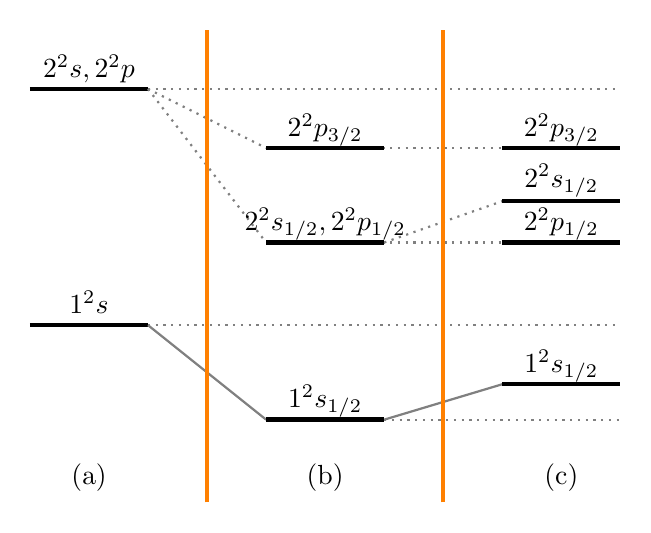
\begin{tikzpicture}[scale=1.5]
% Lines
\draw[black, ultra thick] (1,1) -- (2,1);
\draw[gray, thick, dotted] (2,1) -- (6,1);
\draw[gray, thick] (2,1) -- (3,0.2);
\draw[black, ultra thick] (3,0.2) -- (4,0.2);
\draw[gray, thick] (4,0.2) -- (5,0.5);
\draw[gray, thick, dotted] (4,0.2) -- (6,0.2);
\draw[black, ultra thick] (5,0.5) -- (6,0.5);
\draw[black, ultra thick] (1,3) -- (2,3);
\draw[gray, thick, dotted] (2,3) -- (6,3);
\draw[gray, thick, dotted] (2,3) -- (3,1.7);
\draw[gray, thick, dotted] (3,1.7) -- (6,1.7);
\draw[gray, thick, dotted] (4,1.7) -- (5,2.05);
\draw[black, ultra thick] (5,2.05) -- (6,2.05);
\draw[black, ultra thick] (3,1.7) -- (4,1.7);
\draw[black, ultra thick] (5,1.7) -- (6,1.7);
\draw[gray, thick, dotted] (2,3) -- (3,2.5);
\draw[gray, thick, dotted] (3,2.5) -- (6,2.5);
\draw[black, ultra thick] (3,2.5) -- (4,2.5);
\draw[black, ultra thick] (5,2.5) -- (6,2.5);
\draw[orange, ultra thick] (2.5,-0.5) -- (2.5,3.5);
\draw[orange, ultra thick] (4.5,-0.5) -- (4.5,3.5);
% Nodes
\filldraw[black] (1.5,1.15) node[anchor=mid]{$1^2s$};
\filldraw[black] (3.5,0.35) node[anchor=mid]{$1^2s_{1/2}$};
\filldraw[black] (5.5,0.65) node[anchor=mid]{$1^2s_{1/2}$};
\filldraw[black] (3.5,1.85) node[anchor=mid]{$2^2s_{1/2},2^2p_{1/2}$};
\filldraw[black] (5.5,1.85) node[anchor=mid]{$2^2p_{1/2}$};
\filldraw[black] (5.5,2.22) node[anchor=mid]{$2^2s_{1/2}$};
\filldraw[black] (3.5,2.65) node[anchor=mid]{$2^2p_{3/2}$};
\filldraw[black] (5.5,2.65) node[anchor=mid]{$2^2p_{3/2}$};
\filldraw[black] (1.5,3.15) node[anchor=mid]{$2^2s, 2^2p$};
\filldraw[black] (1.5,-0.3) node[anchor=mid]{(a)};
\filldraw[black] (3.5,-0.3) node[anchor=mid]{(b)};
\filldraw[black] (5.5,-0.3) node[anchor=mid]{(c)};
\end{tikzpicture}
   % \caption{Not to scale sketch of hydrogen energy levels according to (a): Bohr-Sommerfield Theory,  (b): Dirac Theory, and (c): Quantum Electrodynamics}
   % \label{fig:06:lambshiftenergydiagram}
%\end{figure}
\end{document}
